\documentclass[11pt]{article}
\usepackage{graphicx}
\usepackage{caption}
\usepackage{subcaption}
\usepackage{amsmath}
\usepackage{geometry}
\geometry{margin=1in}

\begin{document}

\begin{figure}[htbp]
    \centering
    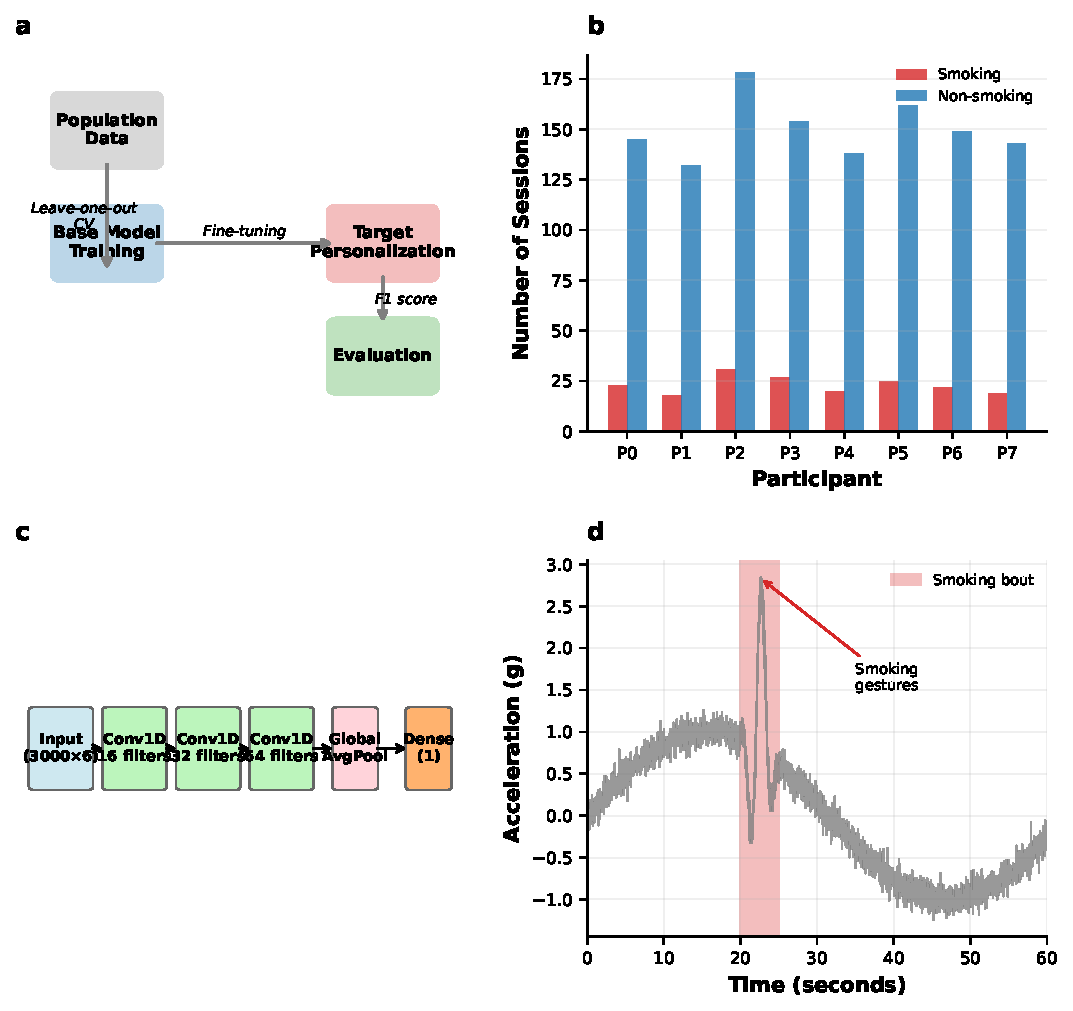
\includegraphics[width=\textwidth]{figures/figure1.jpg}
    \caption{\textbf{Study design, dataset characteristics, and methodology.}
    \textbf{a}, Experimental workflow showing the leave-one-out cross-validation approach for personalization evaluation. Population data from multiple participants is used to train a base model, which is then personalized through fine-tuning on individual target participants' data, followed by evaluation on held-out test data.
    \textbf{b}, Dataset characteristics showing the distribution of smoking and non-smoking sessions across all eight participants (P0-P7). Data collection involved accelerometer recordings at 50Hz, with sessions annotated for smoking behavior.
    \textbf{c}, Model architecture diagram illustrating the lightweight 1D CNN designed for 60-second accelerometer windows (3000 samples × 6 features). The network consists of three convolutional layers with increasing filter counts, followed by global average pooling and a binary classifier.
    \textbf{d}, Representative accelerometer trace showing characteristic patterns during smoking behavior. The highlighted region demonstrates the distinctive hand-to-mouth gestures captured during smoking events, which the model learns to recognize.}
    \label{fig:study_design}
\end{figure}

\section{Methods}

\subsection{Experimental Design}

Our study employed a leave-one-out cross-validation approach to evaluate the effectiveness of personalized smoking detection models (Figure~\ref{fig:study_design}a). For each of the eight participants, we trained a base model on data from the remaining seven participants, then applied different personalization strategies using the target participant's training data. This approach ensures that base models contain no information about the target participant, providing a realistic assessment of personalization benefits.

\subsection{Dataset and Data Collection}

Accelerometer data was collected from eight participants using wearable devices at 50Hz sampling rate (Figure~\ref{fig:study_design}b). Data was organized into 60-second windows (3000 samples per window) and labeled based on smoking bout annotations stored in our database. The dataset exhibits natural class imbalance, with smoking sessions representing approximately 12\% of all recorded sessions across participants. Session durations and smoking frequency varied considerably between individuals, reflecting real-world usage patterns.

\subsection{Model Architecture}

We developed a lightweight 1D convolutional neural network optimized for accelerometer time-series classification (Figure~\ref{fig:study_design}c). The architecture processes 3000-sample input windows corresponding to 60 seconds of 6-channel accelerometer data (x, y, z axes plus derived features). Three convolutional layers with increasing filter counts (16, 32, 64) extract hierarchical temporal features, followed by global average pooling and a binary classifier. This design balances representational capacity with computational efficiency, making it suitable for personalization scenarios requiring multiple model training runs.

\subsection{Data Characteristics and Smoking Behavior}

Accelerometer traces during smoking events exhibit characteristic patterns reflecting hand-to-mouth gestures and device manipulation (Figure~\ref{fig:study_design}d). These behavioral signatures vary between individuals due to differences in smoking style, device placement, and personal habits. The temporal structure of smoking sessions provides rich signal for machine learning models, with distinctive acceleration patterns occurring during cigarette handling, lighting, and consumption phases.

\end{document}